\documentclass{article}
\usepackage{tikz}

\begin{document}
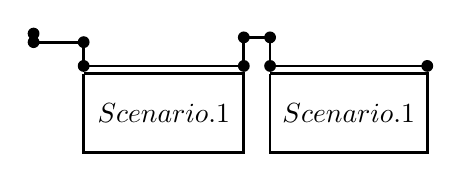
\begin{tikzpicture}
\fill (0, 8.88533) circle (0.075) ; % State.0 
\fill (0, 8.77653) circle (0.075) ; % State.1 
\fill (0.63602, 8.77653) circle (0.075) ; % State.2 
\fill (0.63602, 8.47431) circle (0.075) ; % State.3 
\fill (2.67003, 8.47431) circle (0.075) ; % State.4 
\fill (2.67003, 8.83698) circle (0.075) ; % State.5 
\fill (3.00378, 8.83698) circle (0.075) ; % State.6 
\fill (3.00378, 8.47431) circle (0.075) ; % State.7 
\fill (5, 8.47431) circle (0.075) ; % State.8 
\draw[line width=1pt] (0, 8.88533)  -- (0, 8.77653) ; % TimeNode.0 
\draw[line width=1pt] (0.63602, 8.77653)  -- (0.63602, 8.47431) ; % jazz93sill47 
\draw[line width=1pt] (2.67003, 8.83698)  -- (2.67003, 8.47431) ; % sack61gulf36 
\draw[line width=1pt] (3.00378, 8.83698)  -- (3.00378, 8.47431) ; % herb98oval5 
\draw[line width=1pt] (5, 8.47431)  -- (5, 8.47431) ; % moss21fens52 
\draw[line width=1pt] (0, 8.77653)  -- (0.63602, 8.77653) ; % pegs4duff56 
\draw[line width=1pt] (0.63602, 8.47431)  -- (2.67003, 8.47431) ; % test 
\draw[line width=1pt] (0.63602, 8.37431)  -- (2.67003, 8.37431)  -- (2.67003, 7.37431)  -- (0.63602, 7.37431)  -- (0.63602, 8.37431) ;
\draw (1.65302, 7.87431) node {$Scenario.1$}; % Scenario.1 
\draw[line width=1pt] (2.67003, 8.83698)  -- (3.00378, 8.83698) ; % said71pros73 
\draw[line width=1pt] (3.00378, 8.47431)  -- (5, 8.47431) ; % test2 
\draw[line width=1pt] (3.00378, 8.37431)  -- (5, 8.37431)  -- (5, 7.37431)  -- (3.00378, 7.37431)  -- (3.00378, 8.37431) ;
\draw (4.00189, 7.87431) node {$Scenario.1$}; % Scenario.1 
\end{tikzpicture}

\end{document}
